        %%******************************************%%
        %%                                          %%
        %%        Modello di tesi di laurea         %%
        %%            di Andrea Giraldin            %%
        %%                                          %%
        %%             2 novembre 2012              %%
        %%                                          %%
        %%******************************************%%

\begin{document}
    \frontmatter
    \input{preface/title-page}
    \clearpage
\phantomsection
\thispagestyle{empty}

\hfill
\vfill

\noindent\alberto and \noindent\savas: \textit{\myTitle,}
\myDegree,
\textcopyright\ \myTime.

    % \input{preface/summary}
    % \input{preface/acknowledgements}
    \input{preface/table-of-contents}
    \cleardoublepage

    \mainmatter
    \chapter{Abstract}
\label{cap:abstract}

The recent international expansion of the Bank through the acquisition of other financial entities represents an important opportunity to increase the value of the services provided and achieve several business objectives. However, this expansion also introduces new challenges related to service integration, operational efficiency, regulatory compliance, and the consistent delivery of high-quality IT services across different countries and business units. \\

By analyzing the IT Service Management (ITSM) environment of the Bank presented in the case study, this project supports the strategic transformation of IT Department into a ``Shared Service Center'' thus to operate uniformly, while providing high-quality services across different countries and business units.

Moreover, to achieve business objectives, this document analyzes the individuated Critical Success Factors (CSFs): Customer Partnership, Process Factory, Continuous Improvement. 
Moreover through this document defines different Key Performance Indicators (KPIs), providing a framework template with their respective metric and process involved for the areas identified.
    \chapter{Introduction}
\label{cap:introduction}
    \chapter{Organisational Vision and Goals}
\label{cap:visiongoals}

%   Savas
\section{Vision}
The Banks's organisational vision is focused on business expansion, digital transformation, and international growth. To achieve this vision, the executive board established several objectives, including increasing the domestic retail banking market share from 7\% to 10\%, increasing internet banking revenue by 70\%, increasing revenue generated from customers outside the headquarters country by 50\%, and achieving a 5\% increase in corporate profit. 

The business vison is based on the integration of newly acquired banks, the expansion of strategic partnerships, and the automation and standardisation of business and IT operations. Consequently, Information Technology becomes a strategic enabler rather than a support function. To support the organisational vision, the IT department aims to operate as a Shared Service Center capable of delivering high-performance, high-quality, and cost-effective services. This transformation requires the adoption of a \textbf{Performance-Based Management} approach, where service performance is continuously measured, monitored, and improved through data-driven decision making. The strategic direction of the IT department is therefore built around three Critical Success Factors: Customer Partnership, Process Factory, and Continuous Improvement.


%   Still working on it its gonna grow

\section{Goals}

% • Focus on value 
% • Start where you are 
% • Progress iteratively with feedback 
% • Collaborate and promote visibility  
% • Think and work holistically
% • Keep it simple and practical 
% • Optimize and automate 


The acquisition of foreign banks represents a significant opportunity for the Bank to expand its operations, improve the services provided, and create a more efficient internal organizational structure. This strategic transformation is driven by the objective of increasing value for both the organization and its customers by offering innovative, reliable, and internationally integrated banking services \textit{(focus on value)}.

The IT Department plays a strategic role, by ensuring that business services remains reliable, secure and efficient during this transformation. Thus to accomplish Bank's vision and reach business objectives, the IT Department has adopted the structure of a ``Shared Service Center''; becoming a strategic role, providing not only technical support functions but also delivering standardized, high-quality and cost-effective services across all business divisions.
This centralized approach enables better coordination, reducing duplicated activities and improves service consistency through the organization. The first step is to analyze what logic and process the banks acquired have adopted \textit{(start where you are)}, and to analyze the current IT environment, so identifying existing strengths and weaknesses.


The primary goal of the IT Department is to implement a ``Performance-Based Management'' approach. Through this model, organizational performance is continuously monitored via measurable Key Performance Indicators (KPIs), which provide objective information for decision-making \textit{(progress iteratively with feedback)}. Decisions based on measurable data, rather than subjective opinions enable management to identify weaknesses and monitor progress toward strategic objectives; thus to evaluate the effectiveness of implemented improvements and continuously enhance service quality.

To achieve these strategic objectives, the Bank has identified three Critical Success Factors (CSFs), representing the key areas that require enforcement and attention.

\begin{itemize}
    \item \textbf{Customer Partnership} represnets the first Critical Success Factor. As the Bank expands its international presence and strengthens collaborations with external financial institutions and independent financial advisors, establishing strong relationships with customers and business partners becomes essential \textit{(collaborate and promote visibility)}. The IT Department therefore works closely with business units to actively involve stakeholders throughout the service lifecycle. Through continuous communication, customer feedback and satisfaction surveys, IT can better understand business needs and deliver services that enrich value for customers while supporting the Bank's strategic business.
    As indicated by the corporation and business strategy by the bank:
    \begin{itemize}
        \item In the bank's HQ country, to have as a customer base 10\% of the retail banking market (currently 7~\%)
        \item To increase income from internet banking by 70%
        \item  To increase the income from customers living outside the HQ country by 50\%
        \item To achieve a 5\% increase in corporate profit.
    \end{itemize}

    \item The second Critical Success Factor is \textbf{Process Factory}. The Bank aims to standardize IT processes, technologies, and operational procedures across all acquired organizations and various departments. Standardization reduces complexity, minimizes waste, simplifies maintenance activities and improves service consistency. \\
    Furthermore, standardized processes facilitate the integration of different IT environments and create a clearer workflow of the process, enabiling a more efficeint management of services on an international scale \textit{(keep it simple and practical)}. 
    This objective is particularly important and fragile, since the Bank while maintaining high levels of service quality in multiple countires must ensure different regulations compliance of various nature: Political, Economical, Social, Technological, Environmental and Legal (PESTLE). 
    
    
    \item The third Critical Success Factor is \textbf{Continuous Improvement}. The Bank recognizes that delivering high-quality IT services requires continuous measurement, evaluation and optimization. By collecting and analyzing performance data generated through KPIs, the corporation can identify opportunities for improvement and monitor potential risks.
    The Continuous Service Improvement, reduce operational costs, improve customer satisfaction, optimize resource utilization, and support strategic decision-making based on reliable information. Through incremental improvements, regular feedback, and continuous evaluation of results, the organization can steadily increase the value delivered to customers while optimizing both services and internal resources \textit{(think and work holistically)}.
\end{itemize}


To verify whether these Critical Success Factors are being achieved, the Bank has defined a KPI tree composed of six Key Performance Indicators.


Together, these KPIs provide a balanced overview of service quality, operational efficiency, customer satisfaction and financial performance.
By continuously monitoring these indicators, and where possible, automating the collection and analysis of performances \textit{(optimize and automate)}, the IT Department can ensure that its activities be aligned with overall business strategy.
Furthermore, KPI monitoring supports Service Level Management, enabling the organization to identify areas that require corrective actions and ensure that the service provided accomplish the customer expectations. Moreover, all these procedures ensure the continuous progress toward its strategic objectives. \textit{(keep momentum going)}.



\begin{figure}[h]
    \centering
    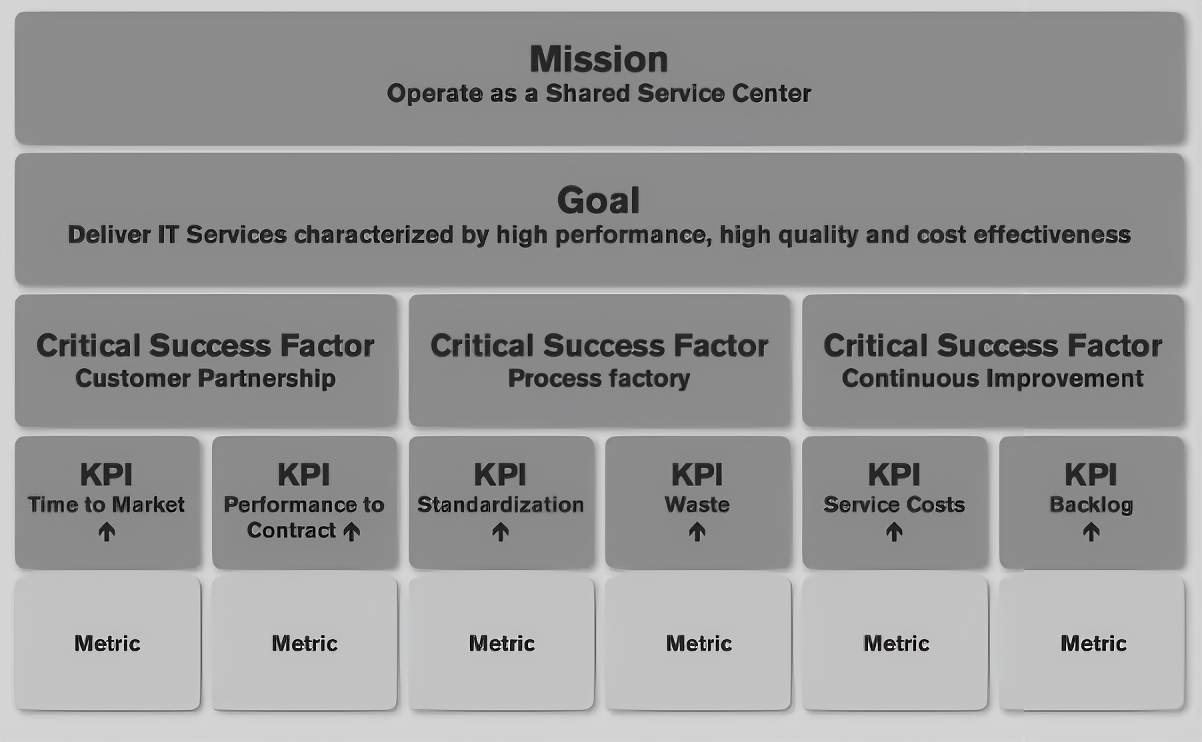
\includegraphics[width=0.8\textwidth]{images/vision.png}
    \caption{what to do}
    \label{fig:whattodo}
\end{figure}

    \chapter{Critical Success Factors}
\label{cap:criticalsuccessfactors}

Critical Success Factors (CSFs) represent the limited number of areas in which satisfactory performance is essential for an organization to achieve its strategic objectives and business goals. Within the context of IT Service Management (ITSM) and Performance-Based Management, CSFs provide a structured mechanism for translating the organization's strategic vision into measurable operational outcomes. They identify the key domains that require continuous attention, monitoring, and improvement to ensure that the organization's mission and strategic objectives are successfully achieved.

For the bank's IT Department, which aims to operate as a Shared Service Center delivering high-quality and cost-effective IT services, Critical Success Factors serve as the foundation for defining performance expectations and establishing appropriate Key Performance Indicators (KPIs). By aligning operational activities, ITSM processes, and performance measurements with these critical areas, the organization can effectively monitor progress, support decision-making, and drive continual service improvement. The following sections analyze each Critical Success Factor individually, identifying the associated KPIs ~\gls{kpi}, suitable metrics, and the ITSM processes that influence their performance. \\

%   SAVAS FIX

\begin{figure}[h]
    \centering
    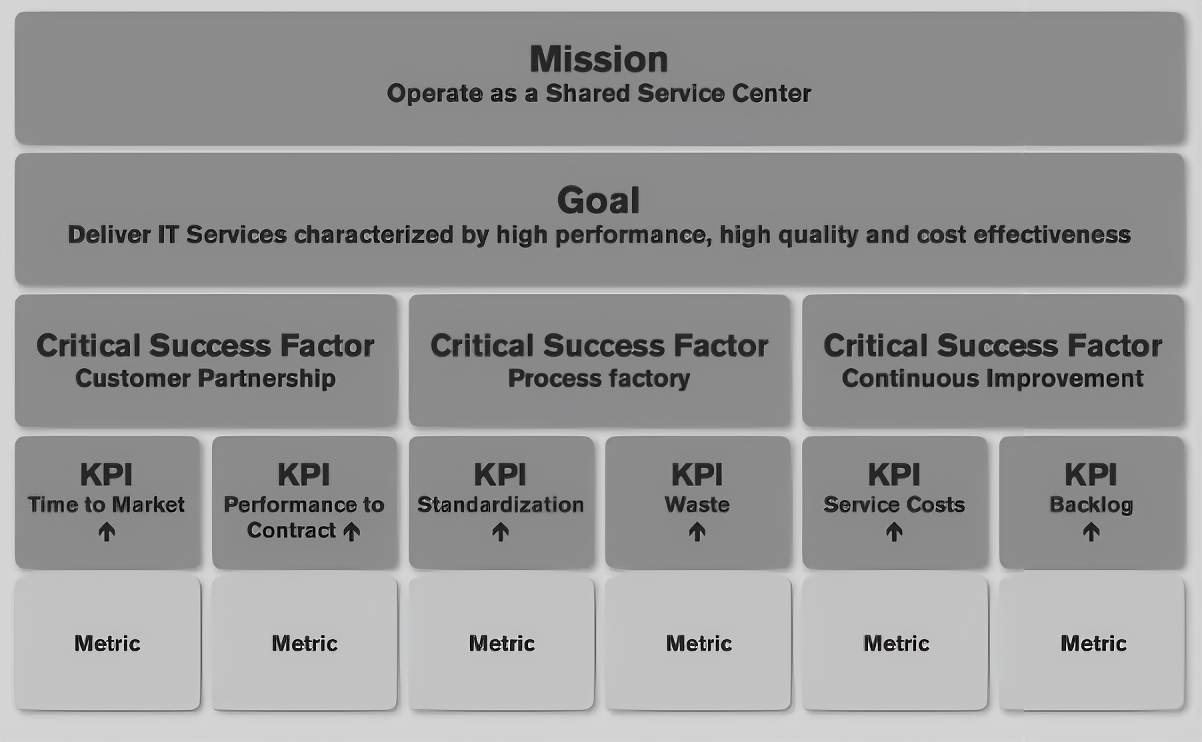
\includegraphics[width=0.9\textwidth]{images/vision.png}
    \caption{Organisational Vision}
    \label{fig:organizational_vision}
\end{figure}


\section{Customer Partnership}

Customer Partnership represents an important and strategic pillar to accomplish the Bank's goals. The IT Department must establish measurable relationships between external customers and other stakeholders, assuming a role that actively contributes to the improvement of the services provided and, in specific, monitors through KPIs ~\gls{kpi} the value perceived by customers.
The IT has to collaborate also internally within the organization in order to engage the appropriate department whenever it is needed.



This topic is fundamental for the success of the Bank's vision, because the international expansion through acquisitions and other partnerships introduces new business requirements due to different customer expectations, cultural diversity, and increased service complexity.
These challenges must be supported in a proactive way, by ensuring that IT services remain aligned with business objectives, deliver consistent value across different countries, and contribute to the Bank's growth, while complying with agreed Service Level Agreements between customers, stakeholders and user expectations.




These requisites, makes performance measurement crucial. By continuously monitoring and collecting customer-oriented metrics and analyzing services scores, IT Department is able to implement a continual service improvements that can strengthen customer trust and enrich the service quality. Gaining long-term partneship.
This customer-centric approach supports organization's objectives of delivering high-performance, high-quality and cost-effective IT services. Aimed toward to accomplish the predefined goals \ref{cap:goals}



\subsection{Time To Market}
\label{subs:timetomarket}
%   Savas

Time to market, also known as Speed to Market is made operational through \textbf{Average Lead Time for Change to Production} KPI\gls{kpi} metric, defines as the elapsed time between formal approval of a business requirement and its deployment into the production environment. This metric is selected because it directly reflects the organization’s ability to translate customer and business demands into operational banking capabilities which is essential for achieving the stated rapid digital service evolution and revenue growth objectives of the organisation. In the context of the strategic goal of the organisation is to increase the income from internet banking, reduced Time to Market provides higher organizational agility and faster delivery of customer targeting features, thus improving market responsiveness and competitive positioning.

There are several ITIL aligned ITSM processes that primarily effects Time to Market:

\begin{itemize}
    \item \textbf{Change enablement} has a direct effect through approval workflows and Risk Management procedures, were excessive governance overhead can result in significant delays.
    \item \textbf{Release and Deployment Management} also effects the indicator  as deployment scheduling , release batching and automation maturity determine how quickly the validated changes end up deployed in the production.
    \item \textbf{Service Validation and Testing} influences Lead Time through test cycle duration and error handling loops, which can create bottlenecks if automation coverage is insufficient.
    \item \textbf{Service Design and Transition} activities also effect indirectly throught the time required for requirement analysis, architectural validation, and coordination of technical dependencies.
\end{itemize}

Overall, inefficiencies or lack of cooperation across these processes will result in the increase of Lead Time, where higher process integration, standardization and automation would reduce it, resulting with the improvement of Time To Market KPI\gls{kpi}.

%   DONE but check

\subsection{Performance To Contract}
\label{subs:performancetocontract}
% PerformanceToContract --> Alberto

Performance to Contract focuses on the IT Department`s ability to respect contractual obligations and consistently deliver services according to the agreements made with customers and explained in natural language in the SLAs. \\

This subject requires IT services to meet the agreed levels of different measurable values, such as availability, reliability, responsiveness, and quality, while ensuring and supporting the Bank's operational and predefined business objectives.


% TODO - make a list of definitions, to take more space?? 
% \begin{itemize}
%     \item \textbf{availability}: 
%     \item \textbf{reliability}:
%     \item \textbf{responsiveness}:
%     \item \textbf{quality}: 
    
% \end{itemize}

Well-defined Key Performance Indicators ensure evidence of whether service targets are being achieved and enable the IT department to identify eventual deviations or deficiencies. This gives a clear input to potential corrective actions or improvements to service performance over time. Moreover, the monitoring of performance against contractual commitments also increases transparency and accountability between IT and different business units or external third-party service providers.


This process is fundamental and very important for the Bank, because many banking services, such as Online Banking, ATMs, global payments, or other third-party services, depend strictly on service levels and regulatory compliance. Also, through a cybersecurity point of view, the respect of performance is fundamental to prevent various cyber-attacks and potential disservices.\\
In addition, being a global Bank, the services must be ensured not only during the local time of the main Headquarters, but the support must be available respecting different cultural scenarios, thus supporting suppliers or international partners.


As a result of continuously measuring contractual performance and acting on the collected data, IT Department can improve service reliability, reduce the risk of SLA breaches and improve the overall customer relationships and partnerships with various stakeholders.


\section{Process Factory}
%   Savas

The Process Factory CSF \gls{csf} approach is required in order to transform the IT department into a Shared Service Center, where IT Services are delivered through standardized, repeatable, and performance-oriented processes. This factor is important considering the bank's international expansion strategy, the integration of acquired oversees banks and the consolidation of support functions within the Shared Services  Division.

%   DONE but check

% From Alberto:
The Process Factory approach aims to standardize IT Service Management (ITSM) processes in order to deliver services with greater efficiency, higher quality, and lower operational costs. Within this approach, one of the primary objectives is the systematic identification and elimination of waste, defined as any activity that consumes resources without creating value for customers or supporting business objectives. Moreover the standardization of process helps the creation of waste and redundant steps or activities....to be continued/reviewed


\subsection{Standardization}
\label{subs:standardization}
%   Savas

The Process Factory critical success factor focuses on establishing highly standardized, efficient, and repeatable processes that enable the IT department to operate as a Shared Service Center. Standardization reduces operational complexity, improves service quality, facilitates integration between organisational units, and enables economies of scale. Within the context of the bank case study, standardization is particularly important due to the ongoing integration of acquired international banks, the use of shared services and the strategic objective of delivering high quality and cost effective IT services. \\

To measure the level of standardization achieved within the IT organization, Percentage of IT Services Complying with Standardized Service and Infrastructure Architectures needs to be used as a KPI\gls{kpi} metric. This metric measures the proportion of IT services that fully conform to the organization's approved standards, including standardized architectures, service designs, infrastructure platforms, operating procedures, and technology stacks. Standardization Compliance Rate provides an indication of the organization's ability to implement consistent and repeatable service delivery practices across business units and geographical regions.

A high value for this metric indicates a mature and efficient operating model characterized by reduced complexity, simplified maintenance activities, improved interoperability, and lower operational costs. This directly supports the bank's strategic objective of integrating international operations while maintaining high service quality and cost effectiveness.

Several IT Service Management processes have a direct impact on the degree of standardization achieved within the organization:

\begin{itemize}
    \item \textbf{Service Portfolio Management:} Ensures that new and existing services align with organizational standards and strategic objectives. Also prevents the introduction of unnecessary service variations.
    \item \textbf{Service Design:} Defines standardized service architectures, technical specifications, support models, and operational requirements. Furthermore promotes the reuse of existing service components and standardized technologies.
    \item \textbf{Change Enablement:} Controls modifications to services and infrastructure, ensuring that implemented changes comply with approved standards. Additionally prevents unauthorized deviations from established architectures.
    \item \textbf{Service Asset and Configuration Management:} Maintains accurate information about service assets and configuration items, enabling verification of compliance with approved standards.
    \item \textbf{Release and Deployment Management:} Ensures that new releases and deployments are implemented using standardized procedures, tools, and configurations.
    \item \textbf{Continual Service Improvement:} Monitors standardization performance metrics and identifies opportunities to further reduce process variation and improve operational efficiency.
\end{itemize}

%   DONE but check

\subsection{Waste}
\label{subs:waste}

With the term \textbf{waste} IT Service Management intend every activioty that consumes time, effort or financial resources without increasing the value delivered to the customer. From Lean methodology and ITIL perspective, customers only perceive value when an IT service is available, reliable, secure and supports the desired utility functions. 
Any process that do not contribute to outcomes is considered waste and should be minimized or eliminated (\textit{as the guiding principles suggests: ``Keep it simple and practical''}).

Waste includes more than obvious failures, such as services outages but also hidden inefficiencies embedded in recurrent operations. These may include redudant processes steps, unnecessary approvals, excessive manual work, repeated incident resolution, but even the collections of data taht is never used to improve services.\\
Such activities increase opreational costs, reducing productivity and delaying service delivery, impact negatively ithe customer satisfaction.

Lean thinking identifies different categories of waste that can be directly applied to IT Service Management, such as:
\begin{itemize}
    \item \textbf{Waiting}: delays caused by approvals, unavailable personnel or dependencies between teams. \textit{Waiting increases lead time without adding value.}
    \item \textbf{Defects}: errors that require correction, like failed software releases, configuration mistakes, security vulnerabilities, or inaccurate service records.
    \item \textbf{Overprocessing}: performing more work than necessary, including excessive documentation not required or needed by stakeholders. Even unnecessary or redundant approvals, or too many resources allocated to simple activities (often wrongly added near to a delivery deadline).
    \item \textbf{Unused talents}: failing to involve employees with valuable expertise in process improvement, service design or decision-making. \textit{Opposing the ``Collaborate and promote visibility'' guiding principle.}
    \item \textbf{Inventory}: backlogs of unresolved incidents, accumulated change requests, unused hardware, and outdated or unused retreived information.
\end{itemize}

These concepts can be applied through concrete examples to the Bank's use case scenario. For instance, without a structured \textbf{knowledge management} that holds documentation and reusable knowledge, service desk analysts and technical staff repeatedly solve the same problems independently. This duplication of effort represents both overprocessing and inventory waste, increasing incident resolution times and reducing overall efficiency.\\
Another source of waste comes from poor involvement of internal customers during the Service Transition and Service Design, as a result a lot of misunderstandings and usability issues could emerge that converge into rework, additional testing, and corrective changes. This represents both waiting and defects of a service, since problems are identified later in the service lifecycle or already in a production environment

An important aspect that the Bank needs to handle, thus avoiding waste, is due to the expansion into different countries. Social aspects such as language, culture, time zones, and organizational practices could end up creating a bottleneck for the communication system, delaying the throughput of information and slowing incident resolution, change approvals, or decision-making.


Even the differences in operational practices, in the absence of standardized processes \ref{subs:standardization}, could represent a duplication of work and the creation of organizational silos, which can slow down decisions taken toward goal realization, representing the opposite of one of \textit{ITIL core guiding principle ``Think and work holistically''}.
For the Bank, reducing waste is a necessity that allows IT resources to focus on innovation, improvements in service quality and lower operating costs. In order to individuate waste, the organization must ensure standardization of processes, automate repetitive activities, define responsibilities and continuously monitor performance through KPIs~\gls{kpi} (analyzed in the following chapter ??). This transformation of strategy makes the IT department operate as a ``Shared Service Center'' that provides high performance, high quality and cost-effectiveness, aligned with the organization's goals.


\section{Continuous Improvement}
\label{sec:continuousimprovement}
%   Savas
Within the bank’s Shared Service Center IT operating model, Continous Improvement represents a critical success factor focused on the systematic and sustained enhancement of IT service performance through structured, data-driven decision-making. It establishes improvement as an embedded capability rather than a set of isolated initiatives, ensuring that IT services, processes, and supporting technologies evolve in alignment with business objectives such as increased internet banking revenue, improved customer reach, and higher operational efficiency. In this context, Continual Improvement is not limited to reactive problem resolution but extends to proactive optimisation of service performance, cost structures, and delivery speed across all IT service management domains.

This CSF \gls{csf} is operationalised through the consistent use of performance metrics, service reporting, and analytical feedback loops that convert operational data into actionable improvement opportunities. In a complex, geographically distributed banking environment with multiple acquired entities, Continual Improvement becomes essential to reduce performance variability, eliminate systemic inefficiencies, and ensure that IT services remain scalable and compliant with regulatory constraints. It also directly supports the bank’s strategic ambition to integrate heterogeneous IT landscapes by promoting standardisation of measurement practices and reinforcing a unified performance management culture across all divisions.

A key characteristic of this CSF\gls{csf} is its dependency on mature measurement and governance capabilities. Improvement decisions are expected to be grounded in quantifiable evidence derived from ITSM processes rather than subjective assessment. As a result, Continual Improvement is tightly coupled with the organisation’s ability to capture reliable service data, analyse trends, and implement corrective actions through controlled change mechanisms. Without this closed-loop structure, improvement efforts risk becoming fragmented, inconsistent, and misaligned with strategic objectives.


\subsection{Service Costs}
\label{subs:servicecosts}
%   Savas

To support the Continuous Improvement critical success factor, the selected metric for the Service Costs key performance indicator is Total IT Service Cost per Service (TISCS). This metric measures the complete financial cost associated with delivering, operating, supporting, and maintaining an individual IT service over a defined reporting period. The calculation includes both direct costs, such as infrastructure, software licensing, personnel, and supplier expenditures, and indirect costs, such as shared facilities, administrative overhead, and common support services.

The selection of Total IT Service Cost per Service as the primary metric is justified by the strategic objective of operating the IT department as a Shared Service Center delivering high-quality and cost-effective services. Unlike traditional budgetary measures, which provide only an aggregated view of expenditure, this metric enables service-level cost transparency and supports informed managerial decision-making. Furthermore, it allows the organization to identify cost inefficiencies, compare service performance across business units and international operations, evaluate the financial impact of improvement initiatives, and optimize resource allocation.

In the context of the case study, this metric is particularly relevant due to the bank's ongoing international expansion, integration of acquired institutions, and increasing reliance on shared services and standardized IT operations. By measuring the total cost of individual IT services, the bank can assess whether service delivery remains economically sustainable while maintaining the required levels of performance and quality. \\

Several IT Service Management (ITSM) processes directly influence the Total IT Service Cost per Service metric. Service Portfolio Management affects the metric by determining which services are offered, maintained, or retired, thereby influencing the overall service cost structure. Financial Management for IT Services plays a critical role in budgeting, accounting, cost allocation, and financial reporting associated with individual services. Service Level Management impacts service costs through the definition of service quality targets and performance requirements, which determine the resources necessary for service delivery. Change Management and Release and Deployment Management influence the metric by affecting the cost of implementing new or modified services and introducing operational efficiencies or inefficiencies. Service Asset and Configuration Management contributes by providing accurate information regarding infrastructure assets and their associated costs. Finally, Continual Service Improvement directly affects this metric through the identification and implementation of initiatives aimed at reducing operational costs, improving efficiency, and increasing the overall value delivered by IT services. \\

Consequently, Total IT Service Cost per Service provides a comprehensive and strategically aligned measure of cost effectiveness, supporting both the bank's Continuous Improvement objectives and its broader transformation towards a performance-based management culture.

%   DONE but check

\subsection{Backlog}
\label{subs:backlog}

%   Alberto

Backlog represnets a structured and prioritized repository of improvements initiatives taken or identified through service performance measurement methods like KPI~\gls{kpi} monitoring, incidents, problem analysis or customer feedback and reviews.
Provide a governance mechanism that enables the organization to systematically collect, evaluate, pripritize and monitor the improvement process and opportunities in a shared system rather than operate as an organizational silos.
In fact, backlog represent a key tool for the transformation of the IT Department into a ``Shared Service Center'', because improvement initiatives are continuously generated from the monitoring of KPI~\gls{kpi} across various processes. The adoption of a welformed backlog gives the IT the possibility to provide and suggest different initiatives thus to ensure the investments of resource and operation that contribute directly to the organization's goals and  support informed decision-making.

Initiatives are prioritized by different factors, such as:
\begin{itemize}
    \item \textbf{Business value} that provide to the customers
    \item \textbf{Strategic alignment} toward organisation's goals
    \item \textbf{Implementation effort}
    \item \textbf{Operational risk}
    \item \textbf{Expected benefits }
    \item \textbf{Resouce ability}
\end{itemize}

The backlog must be continuously reviewed as part of the \textit{Continual Service Improvement} process, allowing new opportunities to be integrated while completed activities can be evaluated against predefined performance indicators.
The outcome of each implemented improvement is measured through opportune KPIs~\gls{kpi} to verify and then support the validation of the achievement of the expected benefits. Moreover, can serve to identify additional optimization and creating a feedback loop that promotes organizational learning and maturity.


Applied to the Bank current ITSM environment, the adoption of an improvement backlog brings several benefits to the services provided, such as:
\begin{itemize}
    \item Enrich and consolidate a Knowledge Management
    \item Increase customer involvement during Service Transition
    \item Introduce formal change evaluation process 
    \item Promote proactive Problem Management
    \item Standardize operational process across international branches and improve collaboration between departments
\end{itemize}

Together, these initiatives contribute the reducing of operational waste while improving service quality, increasing process efficiency and supporting Banks's international growth strategy through a culture of continuous improvement.

    \chapter{Measurement Procedures}
\label{cap:measurementprocedures}


\section{Time to Market}
%   Savas

\section{performance to Contract}
%   Alberto

\section{Standardization}
%   Alberto

\section{Waste}
%   Savas

\section{Service Costs}
%   Alberto

\section{Backlog}
%   Savas
    \chapter{Conclusions}
\label{cap:conclusions}
%   Savas

%   What did we do and whats the impact of the work we did for the company

This work analyses the strategic transformation of the Bank's IT Department toward a ``Shared Service Center'', operating model with the adoption of ITIL principles applyed to IT Service Management processes, and a KPI Based Management approach. \\
The international expansion of the organization, together with the integration of acquired financial institutions and collaboration with indipendent financial advisors, introduces significant challenges related to service standardization, operational efficiency, customer satisfaction, cost management and regulatory compliance. Consequently, the establishment of measurable performance mechanisms becomes essential to support strategic decision-making and ensure the long-term sustainability of IT services. \\
This document analyzed the Critical Successful Factors (\gls{csf}) individuated and provide respective KPI metrics to analyze and measures organizational processes thus to monitor and improve the value provided; as Figure ~\ref{fig:kpimetrics} illustrate, each CSF is composed by two related core topics and respectly the indicators deisgned.

%   Still WIP

\begin{figure}[h]
    \centering
    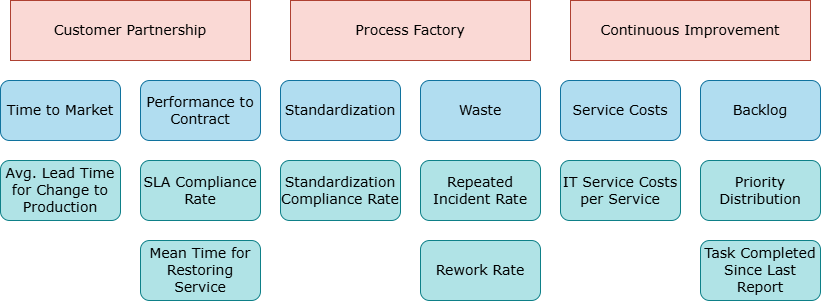
\includegraphics[width=0.8\textwidth]{images/metrics.png}
    \caption{KPI Metrics Relations Table}
    \label{fig:kpimetrics}
\end{figure}

    \appendix
    % \input{appendix/appendice-a}

    \backmatter
    \printglossary[type=\acronymtype, title=Acronimi e abbreviazioni, toctitle=Acronimi e abbreviazioni]
    \printglossary[type=main, title=Glossario, toctitle=Glossario]

    \input{appendix/bibliography}
\end{document}
